\section{Multiplicative Market Share}
\label{sec:beyond-linear}

We next study a multiplicative market share function as another special case of the general model. Multiplicative demand formulations have a long history in promotion research, including the analysis of dynamic promotion effects by \citet{vanheerde2000dips}. \citet{cohen2017promotion} use a product of current and historical price effects in promotion planning. These formulations provide a foundation for studying how proportional effects on demand accumulate across periods.

A practical setting is a subscription or repeat purchase service in which customers may churn before the maximum age \(\mathcal A\). Customers arrive engaged. In each period, an engaged customer renews and purchases at price \(p\) with probability \(s(p)\), and otherwise churns permanently. This gives a Markov chain with two states, engaged and churned, with churned absorbing. Promotions increase retention, so we write \(s(p^L)=s_1\) and \(s(p^H)=s_2\), where \(0<s_2<s_1<1\).

A customer arriving at time \(t-a\) purchases at time \(t\) only if every renewal through age \(a\) succeeds. The resulting market share is
\[
    M_a^{\mathrm{mul}}(p_t,y_{a,t})
    =\prod_{j=0}^{a}s(p_{t-j})
    =s(p_t)s_1^{y_{a,t}}s_2^{a-y_{a,t}}.
\]
The historical factors describe survival up to the current period, and \(s(p_t)\) is the probability of the current renewal. Repeated promotions reinforce demand by preserving a larger customer base for subsequent renewals.

Define
\[
    \theta=\frac{s_1}{s_2},
    \qquad
    \kappa=\frac{p^H}{p^L}.
\]
Replacing a remembered regular price with a promotional price multiplies market share by \(\theta>1\). The ratio \(\kappa>1\) measures the regular price relative to the promotional price. These two ratios determine the curvature of the window revenue contributions.

\subsection{Multiplicative window contributions}

For multiplicative market share, the marginal effect of the \(k\)th remembered promotion is
\[
 \Delta_{a,k}^H=s_2^{a+1}(\theta-1)\theta^{k-1},\qquad
 \Delta_{a,k}^L=\theta\Delta_{a,k}^H,
 \qquad 1\le k\le a\le\mathcal A.
\]
Substituting these effects into Proposition~\ref{thm:exposure-decomposition} gives the window contributions and their second differences. Cohort arrival mass is one, and retention is already incorporated in \(M_a^{\mathrm{mul}}\).

\begin{corollary}[Multiplicative window contributions]
    \label{prop:mult-gamma}
For \(b=1,\ldots,\mathcal A\), define
\[
 S_b^{\mathrm{mul}}(\kappa)=
 \begin{cases}
 s_1(1-s_2)-\kappa s_2(1-s_1),&1\le b<\mathcal A,\\
 s_1-\kappa s_2,&b=\mathcal A.
 \end{cases}
\]
The window revenue contributions are
\[
 F_b(n)=p^Ls_2^bS_b^{\mathrm{mul}}(\kappa)
 \frac{\theta^n-1-n(\theta-1)}{\theta-1},
 \qquad n=0,\ldots,b+1,
\]
and their second differences satisfy
\[
 \psi_{b,k}=F_b(k+1)-2F_b(k)+F_b(k-1)
 =p^Ls_2^b(\theta-1)\theta^{k-1}S_b^{\mathrm{mul}}(\kappa),
 \qquad k=1,\ldots,b.
\]
\end{corollary}

The factor multiplying \(S_b^{\mathrm{mul}}(\kappa)\) in \(\psi_{b,k}\) is positive. Thus, at each depth \(b\), all second differences have the same sign across promotion counts \(k\). Thus \(F_b\) is concave when \(S_b^{\mathrm{mul}}(\kappa)\le0\) and convex when \(S_b^{\mathrm{mul}}(\kappa)\ge0\). These are the shape conditions in Theorem~\ref{thm:general-sign-arrangement}. The derivation appears in \hyperlink{proof-multiplicative-windows}{Section~\ref*{app:mult-regimes}} of the supplementary appendix.

\subsection{Optimal arrangement regimes}

The price and retention ratios determine whether all window contributions are convex, all are concave, or their second differences have mixed signs. These regimes provide sufficient conditions for single block and balanced optimality at a prescribed cycle length and number of promotions.

If \(\mathcal A=0\), there are no terms that depend on arrangement, and all arrangements with the same \((\mathcal T,m)\) earn the same revenue. For \(\mathcal A\ge2\), define
\[
    \tau^{\mathrm{mul}}
    =\frac{s_1(1-s_2)}{s_2(1-s_1)}.
\]
The threshold \(\theta=s_1/s_2\) compares the retention gain from a promotion with its price reduction. The inequality \(\kappa\le\theta\) is equivalent to \(p^Ls_1\ge p^Hs_2\). A promotion then weakly increases expected current revenue from an engaged customer while improving retention. The interior threshold also reflects churn reduction through the identity
\[
    \tau^{\mathrm{mul}}
    =\theta\frac{1-s_2}{1-s_1}
    =\frac{s_1/(1-s_1)}{s_2/(1-s_2)}.
\]
It is the ratio of retention odds under the two prices, and \(\tau^{\mathrm{mul}}>\theta\). At the terminal age, no further renewal remains, so the threshold reduces to the immediate revenue comparison \(\theta\).

\begin{proposition}[Multiplicative arrangement regimes]
    \label{thm:mult-regimes}
Fix a cycle length \(\mathcal T\) and number of promotions \(m\), and suppose \(\mathcal A\ge1\).

\begin{enumerate}[label=(\roman*)]
    \item If \(\kappa\le\theta\), every \(F_b\) is discretely convex, and a single block cycle is optimal.
    \item Every \(F_b\) is discretely concave if and only if \(\kappa\ge\tau^{\mathrm{mul}}\) when \(\mathcal A\ge2\), or \(\kappa\ge\theta\) when \(\mathcal A=1\). Under these conditions, every balanced cycle is optimal.
    \item For the remaining parameter values, \(\mathcal A\ge2\) and \(\theta<\kappa<\tau^{\mathrm{mul}}\). The interior contributions \(F_b\), \(b<\mathcal A\), are strictly convex, while \(F_{\mathcal A}\) is strictly concave.
\end{enumerate}
\end{proposition}

When \(\kappa\le\theta\), the retention gain covers the immediate price reduction, and convex window contributions favor concentrating promotions. For \(\mathcal A\ge2\), when \(\kappa\ge\tau^{\mathrm{mul}}\), concave window contributions favor spreading promotions because concentrating discounts on a customer base already enlarged by earlier promotions becomes less attractive. These are the two cases of Theorem~\ref{thm:general-sign-arrangement}. In the region with mixed second-difference signs \(\theta<\kappa<\tau^{\mathrm{mul}}\), a promotion reduces immediate expected revenue but retention benefits make the interior window contributions convex, while the terminal window contribution is concave. The resulting tradeoff requires evaluation of the full revenue objective. The proof appears in Section~\ref{app:mult-regimes} of the supplementary appendix.
\begin{figure}[ht]
    \centering
    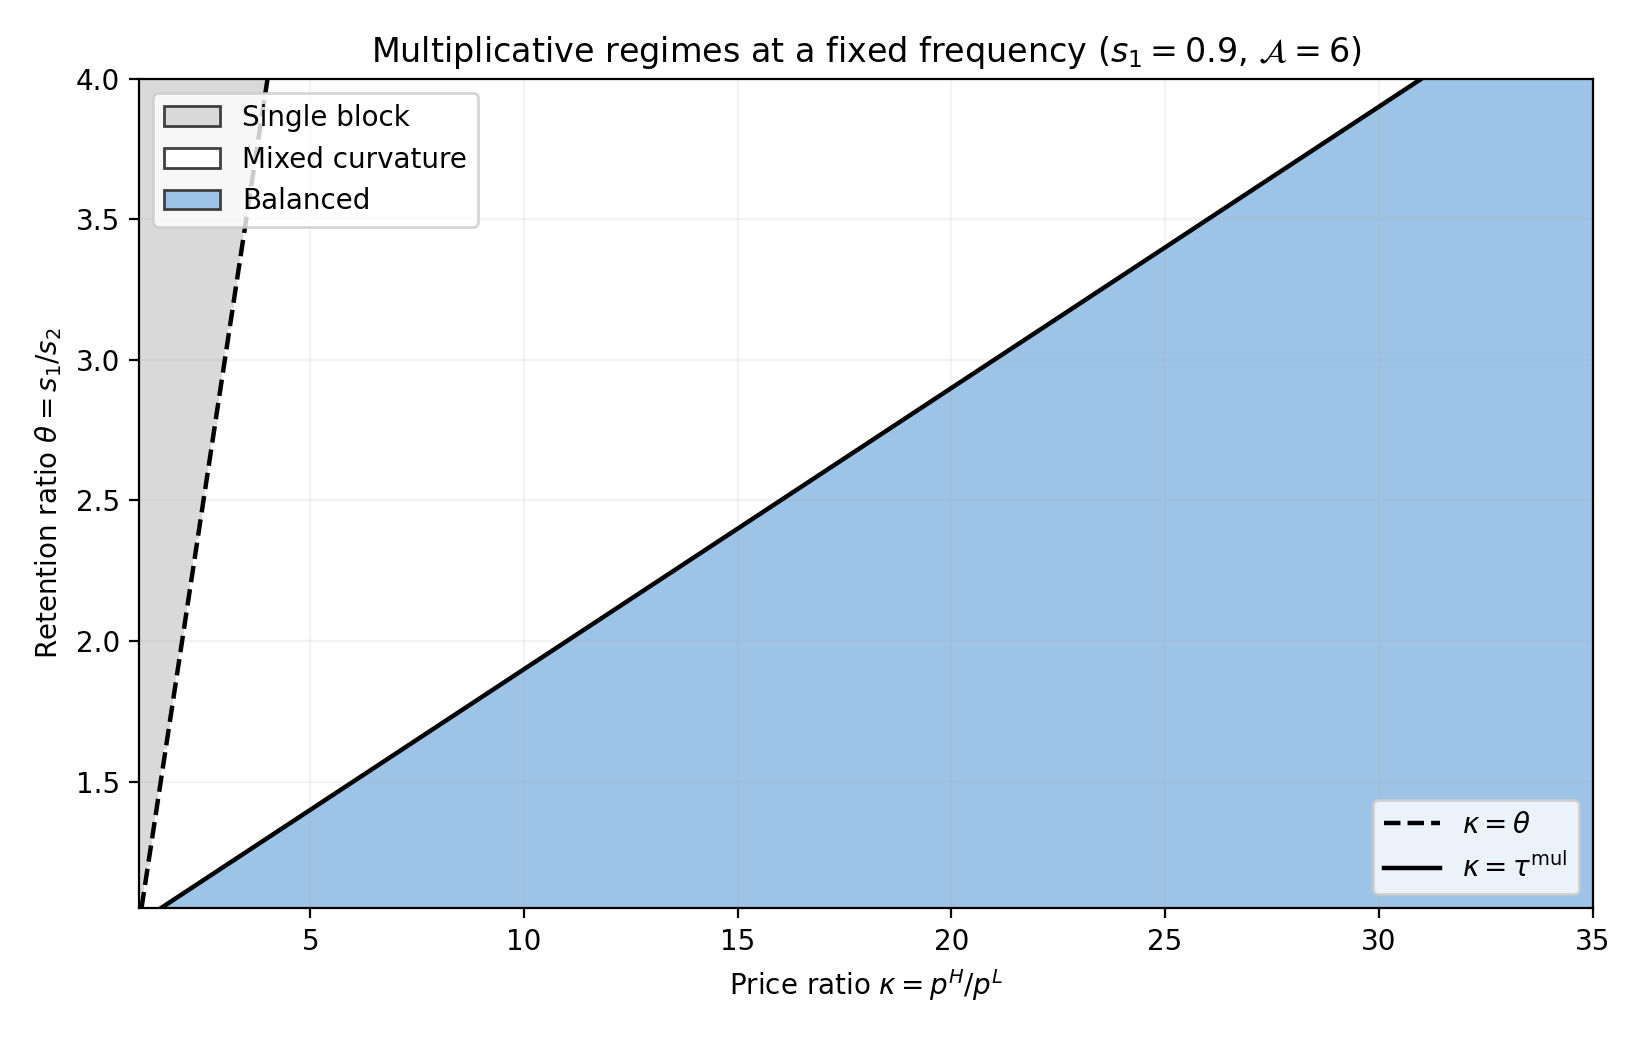
\includegraphics[width=0.68\textwidth]{exp1_phase_diagram.png}
    \caption{Sufficient arrangement regimes from Proposition~\ref{thm:mult-regimes} for prescribed \((\mathcal T,m)\), with \(s_1=0.9\) and \(\mathcal A=6\). The dashed line is \(\kappa=\theta\), and the solid line is \(\kappa=\tau^{\mathrm{mul}}\). In the unshaded region, the interior contributions are convex and the terminal contribution is concave, so neither uniform shape condition applies.}
    \label{fig:mult-regimes}
\end{figure}

For frequency optimization, the conclusions of Propositions~\ref{prop:general-cluster-frequency} and~\ref{thm:pwl} apply directly. Figure~\ref{fig:mult-regimes} illustrates these regimes for \(s_1=0.9\) and \(\mathcal A=6\). In the region with mixed second-difference signs, the uniform concavity or convexity conditions do not apply, and the full revenue objective determines the optimal cycle.
Section~\ref{sec:approximation} bounds the losses of simple policies in this region, and Section~\ref{sec:general-truncation} gives general and multiplicative memory truncation guarantees.

\FloatBarrier
